\documentclass[magd,floatypics,numeref]{msudipl} % класс выбран report, как наиболее подхоящий по структуре и оформлению

%%	ОПИЦИИ КЛАССА msudipl
%%	по умолчанию титульный лист компилируется как курсовая работа
%%	bacw - для бакалаврских работ
%%	magd - для магистерских диссертация
%%	spec - для дипломов специалистов
%%
%%	Оформление литературы
%%	Доступно в основе своей несколько стилей ссылок по действующему ГОСТ Р 7.1-2008
%%	numeref - числом [N], список не сортируется, нумерация сплошная, в порядке упоминания (по умолчанию)
%%	footnotefer - сноской, в сноске краткие сведения, затекстовый список сортируется
%%	authoryear - [Фамилия, год], затекстовый список сортируется
%%	inlineref - (полная запись) - внутритекстовые записи, затекстовый список сортируется
%%	harvard - (Фимиля, год) - Harvard Ref Style, противоречит ГОСТу, затекстовый список будет не по ГОСТ, лучше не пользоваться
%%
%%	Иточники сортируются по языку (и работает \iflitsort). 
%%	Язык указывается в записях в bib-файле в поле langid в каждой записи.
%%	Литература работает на biblatex, см. в шаблоне, как сделать руками что, например, вывод источников по типу.
%%
%%	ТИТУЛЬНЫЙ ЛИСТ
%%	название факультета, можно использовать \par или \\ для красоты
%%	\facname{футурологический факультет}
%%	чтобы убрать название факультета с титульного листа использовать
%%	опцию nofac (исчезнет также и название кафедры)
%%
%%	название кафедры, можно использовать \par или \\ для красоты
%%	\kafname{кафедра вакуумной акустики}
%%
%%	тема ВКР
%%	\diplotitle{что я сделал со своей жизнью}
%%	ФИО студента
%%	\author{Имяреков Имярек Имярекович}
%%	группа
%%	\group{X14}
%%	научники (пишем сколько их надо, редко больше одного)
%%	\supervisor{Мимокрокодилов Антиох Рамзесович}
%%	\supervisor{Случайнопроходилов Киба Тутанхамонович}
%%
%%	Титульный лист продуцируется \maketitle
%%


\usepackage{lscape}					% Для включения альбомных страниц
\usepackage{multirow,makecell,array}		% Улучшенное форматирование таблиц
\usepackage{ dsfont }
\graphicspath{ {./figs/} } %а в эту подпапку будем класть картинки, чтобы не захламлять основную директорию, и да, такой синтаксис в Windows работает

\addbibresource{thesis.bib} 		% Бибилиография, читаем про biblatex

%% ОФОРМЛЕНИЕ ОГЛАВЛЕНИЯ
\setcounter{tocdepth}{2}				% Оглавлении будут только главы и параграфы, но не будет мелких заголовков. Для дипломов нормально, для диссертаций стоит раскомментировать.



% реализация висячей пунктуации, соответствующей традиции русской типографской вёрстки
\usepackage{microtype}
\SetProtrusion
{
encoding = T2A,
family = ftm    %тут указываем тот шрифт, который непосредственно используется. по-умолчанию это faq, но мы выше, после вызова pscyr, выбрали этот шрифт
}
{
« = {1000,   },         %формат команды простой (если вам зачем-то понадобится ещё): _символ_ = {_снос влево в промиле от ширины символа, когда символ стоит в начале строки_ . _снос вправо, когда символ стоит в конце строки_ }
» = {  , 1000},
„ = {1000,   },
“ = {  , 1000},
( = {1000,   },
) = {  , 1000},
! = {  , 1000},
? = {  , 1000},
: = {  , 1000},
; = {  , 1000},
. = {  , 1000},
- = {  , 500},
{,}= {  , 1000}
}
\DeclareMicrotypeSet{t2atext}{encoding=T2A}
\UseMicrotypeSet{t2atext}


\begin{document}
%ТИТУЛЬНЫЙ ЛИСТ
\facname{физический факультет}
\kafname{кафедра физики космоса}
\diplotitle{Стерео-подход комплекса TAIGA к наблюдениям гамма-источника в туманности Dragonfly}
\author{Разумов Александр Юрьевич}
\group{214м}
\supervisor{д.ф-м.н., проф. Кузьмичёв Леонид Александрович}
\maketitle
%КОНЕЦ ТИТУЛЬНОГО ЛИСТА

%\setcounter{page}{2}  % строго говоря, титульный лист обычно за страницу не считается, как и форзацы, но в академических работах всё иначе и считаются даже ПУСТЫЕ страницы, так что нумерация начинается с 2.

\tableofcontents   %вставка оглавления

\phantomsection
\chapter*{Введение}   %добавляем главу "введение" БЕЗ номера, как это положено по правилам
\addcontentsline{toc}{chapter}{Введение}  
%и добавляем её в оглавление, чтобы она там была. 
%синтаксис такой \addcontentsline{в какой автособираемый список: оглавление, список рисунков, список ссылок, список таблиц и пр.}{какого уровня? для оглавления это "глава", "раздел", "параграф" и пр}{какой текст отобразить}. Формально добавить можно в любом месте любую ссылку на это место из соответствующего списка
Целью настоящей работы является поиск гамма-сигнала из туманности Dragonfly по данным черенковских телескопов IACT обсерватории TAIGA с помощью стереоскопического метода, широко применяющегося в такого типа проектах. 

В отличие от заряженных частиц космических лучей, $\gamma$-кванты не меняют своей траектории при прохождении через галактические магнитные поля, сохраняя, таким образом, информацию об источнике их происхождения. Это даёт возможность исследовать астрофизические процессы сверхвысоких энергий. Для изучения астрофизических источников в $\gamma$-диапазоне, а также для общего исследования первичного космического излучения в энергетическом диапазоне свыше нескольких~ТэВ, применяются одни и те же методы наземной регистрации. При этом регистрируется не сама частица, а продукты каскадного рождения вторичных частиц, вызванного прохождением первичной частицы через атмосферу. Выбор источника HWC J2019+368 в туманности Dragonfly в созвездии Лебедь обусловлен его энергетическим спектром, полученном при раннем его исследовании проектами VERITAS и HAWC. При энергиях $E~\geq~10$~ТэВ поток $\gamma$-квантов от источника становится сравним с их потоком от Крабовидной туманности, а энергетический спектр при этом простирается выше 100~ТэВ, что также делает HWC J2019+368 одним из мощнейших источников в галактике, а также потенциальным  <<пэватроном>> --- источником космических лучей с энергиями $E\geq10^{15}$~эВ. Сложность выделения гамма-сигнала вызвана огромным фоном со стороны космических лучей. Задача подавления фона может быть частично решена с помощью стереоскопических наблюдений на черенковских телескопах.

Комплекс TAIGA --- действующая наземная гамма-обсерватория, располагающаяся в Тункинской долине, способная вести наблюдения за гамма-источниками как совместно двумя атмосферными черенковскими телескопами IACT (стереоскопический режим), так и в совпадении с широкоугольными черенковскими телескопами TAIGA-HiSCORE, распределёнными на площади приблизительно~1~$\text{км}^{\text{2}}$ (гибридный режим).
Имеется приблизительно 80~ч данных наблюдения источника из туманности Dragonfly двумя телескопами TAIGA-IACT за осенние сезоны 2020--2021 гг. Приблизительно 45~ч из этих данных соответствуют стереоскопическому режиму наблюдения.

Для достижения поставленной цели требуется решить ряд задач, а именно:
\begin{itemize}
\item Изучить опыт других гамма-астрономических проектов по наблюдению в выбранном энергетическом диапазоне, что представлено в главе 1. 
\item Оценить возможности комплекса TAIGA  по наблюдению выбранного источника, чему посвящена глава 2. 
\item Используя моделирование Монте-Карло решить задачу подавления адронного фона с помощью введения порогов на параметры наблюдаемых изображений, получаемых с телескопов, а также с помощью алгоритма случайного леса из области классического машинного обучения. Этим задачам посвящены главы 3 и 4.
\item Провести обработку данных за осенние сезоны наблюдений 2020--2021 гг и сравнить результаты с предварительными оценками. Поиску гамма-сигнала в обработанных данных посвящена глава 5. 
\end{itemize}


\chapter{Литературный обзор}
\section{Космические лучи}
\subsection{Основные сведения}
Космические лучи являются одним из источников информации о физических процессах, проходящих во Вселенной, и о свойствах межзвёздной среды. Прошло больше ста лет с проведения экспериментов Виктора Гесса, результатом которых было обнаружение роста ионизации воздуха с набираемой высотой. На основании этого, Гесс заключил, что из космоса идёт поток ионизирующего излучения, пронизывающий атмосферу Земли. Впоследствии Роберт Милликен предложил называть это излучение космическими лучами.

В настоящее время к космическим лучам относят заряженные субатомные частицы: протоны, электроны, тяжёлые ядра, галактического и внегалактического происхождения. Диапазон энергий первичных космических лучей простирается от $10^6$ до $10^{21}$~эВ. На протяжении всей истории их изучения пока нет окончательной теории происхождения космического излучения, объясняющей экспериментально наблюдаемые
\begin{itemize}
\item форму энергетического спектра,
\item полную энергию космических лучей,
\item постоянную во времени интенсивность галактических космических лучей,
\item химический состав.
\end{itemize}

Заряженные частицы подвержены влиянию со стороны электромагнитных полей в галактике: электрические поля меняют их энергию, магнитные --- направление полёта. На заряженные частицы в магнитном поле действует сила Лоренца:
\begin{equation}
\vec F = q\left[\vec v\times \vec B\right],
\end{equation}
где $q$ --- электрический заряд частицы, $\vec v$ --- вектор скорости, $\vec B$ --- вектор магнитной индукции. Сила Лоренца действует перпендикулярно движению частицы, тем самым изменяя её траекторию. Радиус кривизны траектории, также называемый ларморовским радиусом или гирорадиусом, равен
\begin{equation}
r_g = \frac{p_{\bot}}{|q|B},
\end{equation}
где $p_{\bot}=\gamma m v_{\bot}$ --- перпендикулярная движению составляющая импульса частицы, $\gamma$ --- Лоренц-фактор частицы. Из-за воздействия магнитных полей становится практически невозможно получить информацию о процессах, происходящих с космическими лучами в их источниках и межзвёздном пространстве. Протон с энергией $E=10^{17}$~эВ при значении галактического магнитного поля $B=10^{-5}$~Гс будет иметь гирорадиус $r_g=$10~пк, что соразмерно с поперечными размерами галактики. Космические лучи с $E<10^{17}~$эВ не несут информации об их происхождении. 
\subsection{$\gamma$-кванты как источник информации}
В отличие от протонов $\gamma$-кванты не имеют заряда и распространяются по галактике без отклонения магнитным полем. Внутри галактики они возникают в остатках сверхновых (SNR), пульсарных туманностях (PWN, плерионы), пульсарах, двойных системах. 
Основные механизмы рождения $\gamma$-квантов в этих источниках в диапазоне энергий от ГэВ~до~ТэВ связаны и с адронами космических лучей, и с электронами. Электроны участвуют в процессах обратного комптоновского рассеяния (IC) и тормозного излучения. Обратное комптоновское рассеяние происходит при взаимодействии высокоэнергичных электронов и мягких фотонов изотропного реликтового микроволнового фона. Тормозное излучение возникает в присутствии плотной среды, например, в молекулярных газовых облаках. В обоих процессах релятивистский электрон $e^-$ взаимодействует с мягким фотоном $\gamma_{soft}$, отдавая ему часть своей энергии. В результате электрон лишается части энергии ($e^{-*}$), а фотон переходит в гамма-диапазон:
\begin{equation}
e^- + \gamma_{soft} \rightarrow e^{-*} + \gamma_{TeV}
\end{equation}

Рождение $\gamma$-квантов происходит и в процессах взаимодействия адрон-адрон (протон-протон). Ускоренный протон космических лучей~$p_{CR}$ может испытать неупругое столкновение с протоном~$p_{ap}$ из окружающей среды. Взаимодействие порождает вторичные частицы, среди которых может оказаться нейтральный пион~$\pi^0$, среднее время жизни которого составляет $t=(8,4\pm0,6)\cdot10^{-17}~$c. Пион распадается на два гамма-кванта с одинаковыми энергиями:
\begin{equation}
p_{CR}+p_{ap}\rightarrow\pi^0+X\rightarrow \gamma+\gamma.
\end{equation}

Вклад того или иного процесса характеризуется временем охлаждения $\tau~=~E/(dE/dt)$. Для четырёх механизмов потери энергии (синхротронные потери, обратный эффект Комптона, тормозное излучение, взаимодействие протон-протон) времена охлаждения определяются как:
\begin{align}
\tau_{sync} = \frac{E_e}{4/3 \,\sigma_T~c~U_{mag} \gamma^2}~\text{[с]}, \\
\tau_{IC} = \frac{E_e}{4/3 \,\sigma_T ~c~U_{rad}   \gamma^2}~\text{[с]}, \\
\tau_{brem} = \frac{X_0}{\rho~c}~\text{[с]}, \\
\tau_{pp} = \frac{1}{n_H \,\sigma_{pp}~c~f}~\text{[с]},
\end{align}
где $\sigma_T$ --- сечение томсоновского рассчения, $c$ --- скорость света,  $U_{mag}~=~B^2/2\mu_0$ --- плотность энергии магнитного поля, $U_{rad}$ --- плотность энергии электромагнитного поля, $\beta^2~=~v^2/c^2$, лоренц-фактор частицы $\gamma^2~=~1/\sqrt{1-\beta^2}$, $X_0$ --- радиационная длина в единицах радиационной длины для данной среды, $n_H$ --- концентрация газа в среде, $\sigma_{pp}$ --- сечение неупругого $pp$-рассения и $f = \Delta E/E$ --- доля энергии, теряемой во взаимодействии. 

\begin{figure}[th]
	\noindent\centering{
		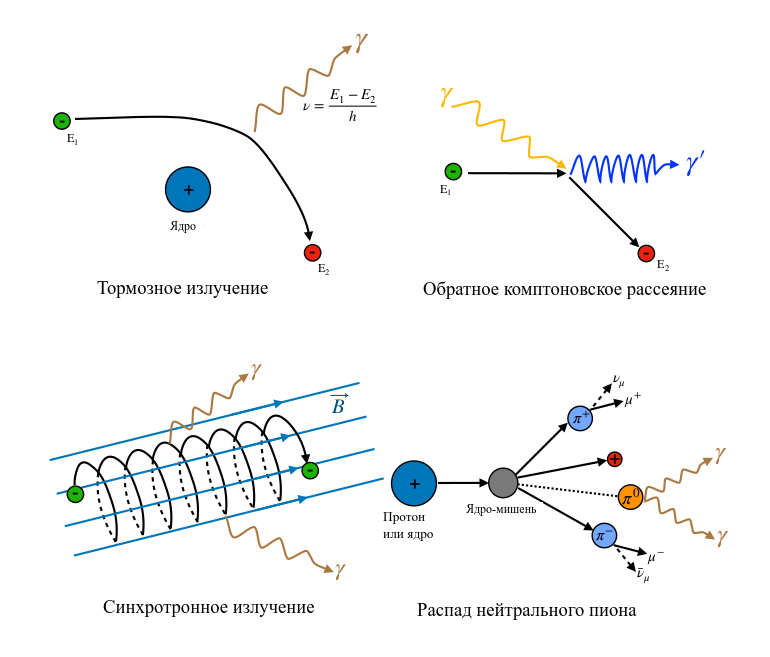
\includegraphics[width=120mm]{figs/four_mechanisms.png}
	}
	\caption{Четыре механизма возникновения $\gamma$-квантов}
	\label{pic:four_mechanisms}
\end{figure}

И синхротронные потери, и обратное комптоновское рассеясние сильно зависят от энергии, и чем больше энергия, тем меньше время охлаждения для обоих процессов.  Если среда обладает сильным магнитным полем, синхротронные потери будут доминировать. Продуктом синхротронных потерь являются фотоны рентгеновского диапазона. С падением магнитного поля начинают доминировать потери энергии электрона на обратное комптоновское рассеяние, порождающее, как сказано ранее, кванты $\gamma$-диапазона. 
В средах с высокой плотностью и слабым магнитным полем доминирующим процессом генерации $\gamma$-квантов в от электронов становятся потери на тормозное излучение. 
\subsection{Пульсары и пульсарные туманности, остатки Сверхновых}
Звёзды с массами от 10 до 30 масс Солнца на финальной стадии своей эволюции претепевают коллапс ядра, сопровождающийся вспышкой Сверхновой. Образовавшийся при этом компактный объект (масса равна 1,4--3~солнечным массам, радиус составляет 10--15~км) называют нейтронной звездой. В процессе взрыва сохраняются магнитный поток $\Phi_B=BR^2$ и момент импульса $L = I\omega$. Здесь $I$ --- момент инерции звезды, $B$ --- индуктивность магнитного поля, $R$ --- радиус объекта, $\omega$ --- угловая скорость вращения. И $\omega$, и $B$ обратно пропорциональны квадрату радиуса $1/R^2$, из-за уменьшения которого  величины колоссально возрастают. Вращающиеся нейтронные звёзды обладают сильным магнитным полем, наклонённым к оси вращения и называются пульсарами, т.\,к. они являются источниками приходящего на Землю электромагнитного излучения с определёным периодом от 1~мс до 10~с. 

Заряженные частицы попадают в магнитные ловушки, ускоряются на силовых линиях пульсара и претерпевают изгибное излучение\footnote{Synchrotron-curvature radiation, один из механизмов синхротронного излучения, связанный с движением релятивистской частицы по искривлённой траектории, радиус кривизны $R_C$ которой определяется магнитным полем.}, из-за чего и возникают $\gamma$-кванты непосредственно от пульсара (\textit{Ссылка на Aliu et al}). 

Вещество сброшенной оболочки звезды сталкивается с межзвёдной средой, и возникает стоячая ударная волна, на фронте которой электроны и позитроны испытывают тормозное и сихротронное излучения, а адроны --- неупругое столкновение с последующим рождением пионов. Этот источник $\gamma$-квантов относят к классу остатков Сверхновых (Supernova remnant, SNR).

Энергия вращения пульсаров теряется на генерацию ветра из ультрарелятивистских электронов и позитронов, впоследствии взаимодействующего с ударной волной. Область взаимодействия, постоянно подпитываемую электрон-позитронным ветром со стороны нейтронной звезды, называют \textit{пульсарной туманностью} (Pulsar Wind Nebula, PWN), или \textit{плерионом}.

\section{Черенковское излучение}
Идея о том, что электрон, передвигаясь в прозрачной среде, будет вызывать излучение с коническим фронтом, была высказана ещё Оливером Хевисайдом (\textit{ссылка}).
Позже, к аналогичным результатам (\textit{ссылка}) пришёл и Арнольд Зоммерфельд, делая расчёты движения заряда со скоростью выше скорости света в вакууме\footnote{Необходимо помнить, что в это время скорость света не считалась принципиальным пределом скорости тел. Более того, движение такого заряда в среде с оптическим показателем преломления $n$ давало решение, не противоречащее результатам СТО}. 

Первое упоминание голубого свечения в экспериментах наблюдалось в работах Марии Склодовской-Кюри (\textit{ссылка}), однако этому эффекту не было придано значение. Дж.\,Джелли указывает на то, что первыми систематическими наблюдениями этого эффекта можно считать исследования Маллета, проведённые ориентировочно в 1926--1928. (\textit{ссылка на Джелли}). Им был, в частности, обнаружен непрерывный спектр излучения, что противоречило предположению Кюри о люминисцентной природе явления, но ключевые свойства излучения, такие как поляризация и анизотропия, не были им установлены. 

П.\,А.~Черенков, будучи аспирантом С.\,И.~Вавилова, обнаружил неизвестное свечение голубоватого света в прозрачных жидкостях под воздействием $\gamma$-излучения солей урана в 1934~г (\textit{ссылка}). Позже, в 1937~г., в работе И.\,Е.~Тамма и И.\,М.~Франка (\textit{ссылка}) была объяснена природа явления, впоследствии названного излучением Вавилова-Черенкова. Согласно их теории, свет испускается средой, через которую проходит заряженная частица со скоростью, превышающей скорость света $v=c/n$ в данной среде (где $c$ — скорость света в вакууме, а $n$ --- коэффициент оптического преломления). 
Дальнейшие эксперименты показали, что:
\begin{itemize}
\item спектр излучения и интенсивность не зависят от чистоты вещества и
температуры;
\item излучение связано с движением электронов в среде;
\item свет поляризован и направлен под небольшим углом к направлению
пучка электронов;
\item эффект имеет пороговый характер, так как не вызывается, например,
электронами, рождёнными в веществе под действием рентгеновских
лучей;
\item спектр излучения непрерывен в излучаемом диапазоне длин волн.
\end{itemize}
В 1958~г. П.\,А.~Черенков, И.\,Е.~Тамм и И.\,М.~Франк получили Нобелевскую Премию за открытие и истолкование эффекта Вавилова-Черенкова.

\section{История развития черенковской гамма-астрономии}
\subsection{Черенковское свечение атмосферы}
В 1948~г. Патрик Блакетт оценил (\textit{ссылка}), что доля в $10^{-4}$ всего света в ночном небе может приходиться на черенковское свечение, возникающее в атмосферных ливнях, порождённых космическими лучами. В 1952~г. Гэлбрейт и Джелли создали установку (\textit{ссылка}), состоявшую из параболического зеркала диаметром 25~см и двух ФЭУ в фокусе зеркала. Раз в минуту <<телескоп>> срабатывал в совпадении с квадратным массивом из 16 счётчиков Гейгера-Мюллера, каждый из которых имел площадь 200~$\text{см}^2$. В результате эксперимента было установлено, что б\'ольшая часть срабатываний установки на световой импульс напрямую коррелирует с регистрацией частиц ШАЛ. Спустя год установка была усовершествована, а также стало возможным исследовать поляризацию света. Было обнаружено, что в регистрируемых вспышках преобладала синяя часть спектра, что также играло роль в пользу гипотезы о черенковском свечении атмосферы.  

В 1953--1955~гг командой под руководством А.\,Е.~Чудакова проводились систематические измерения пространственного распределения черенковского излучения в горах Памира на высоте около 3800~м над уровнем моря (\textit{ссылка}).

Успех обоих экспериментов и идея о том, что ШАЛ могут быть инициированы не только адронами, но и $\gamma$-квантами высоких энергий, стимулировали дальнейшие эксперименты по регистрации $\gamma$-излучения космического происхождения с помощью эффекта Вавилова-Черенкова. 
\subsection{Первые опыты}
В 1958~г. Филип Моррисон предложил вести баллонные измерения  (\textit{ссылка}) потоков $\gamma$-квантов в энергетическом диапазоне 0,2--400~МэВ от возможных источников космических лучей, так как нейтральное  $\gamma$-излучение не отклоняется межзвёздным магнитным полем. В качестве возможного источника $\gamma$-лучей Моррисон рассматривал Крабовидную туманность, предполагая, что в расширяющейся газовой оболочке туманности может быть множество радиоактивных элементов. По его оценке, можно зарегистрировать поток $\gamma$-лучей от $^{226}\text{Ra}$ в~$10^{-2}~\frac{1}{\text{см}^2\cdot\text{с}}$.

В 1959~г. Джузеппе Коккони предложил  (\textit{ссылка}) конструкцию высокогорной установки по регистрации космических лучей и $\gamma$-квантов с~ТэВ-ными энергиями с угловым разрешением в~$1^\circ$. Также он выдвинул оптимистичное предположение о том, что поток $\gamma$-квантов от Крабовидной туманности может быть приблизительно в $10^3$  выше фона. Даже в том случае, если его оценка оказывается слишком оптимистичной, он допускал, сигнал от Крабовидной туманности всё ещё может быть зарегистрирован на земле таким способом. 

В 1960~г. была запущена система из 4 телескопов в на Крымском полуострове на берегу Чёрного Моря, разработка велась командой А.\,Е.~Чудакова. Позже число телескопов было увеличено до 12. Каждый телескоп представлял из себя параболическое зеркало диаметром 155~см и фокусным расстоянием 60~см; в фокус были помещены ФЭУ с диаметром 4,5~см. Выработка триггера для регистрации события просходила в случае четырёхкратного совпадения регистрации на четырёх телескопах. Средний темп счёта атмосферных событий был немного выше  3 Гц. В течение ночи каждые 7~минут шло сопровождение источника телескопом с точностью в $0,2^{\circ}$ по наклонению и $0,4^{\circ}$ по азимуту.

В то время не было никакого представления о пульсарах и их периодах, а также об источниках космического рентгеновского излучения, поэтому выбор источников для наблюдения был обусловлен надеждой на то, что источники радиоизлучения также могут быть и источниками $\gamma$-квантов. Внушительный список исследованных источников включает в себя Крабовидную туманность, Cygnus A, Cassiopeia A, Virgo A, Perseus A, Sagittarius A. 

На сегодняший момент нам известно, что интегральный поток $\gamma$-квантов от Крабовидной туманности с энергиями выше 4~ТэВ составляет приблизительно~$2,5\cdot10^{-12}~\frac{\text{фотонов}}{\text{см}^2\cdot\text{с}}$, однако верхний предел потока, поставленный Чудаковым и командой, был в 20~раз выше этой величины при суммарном времени измерения Крабовидной туманности около 5,5~ч. Это означает, что для обнаружения значимого сигнала от источника им было необходимо было вести измерения в течение минимум 2200~ч.

Важным следствием отсутствия сигнала стала переоценка потока, заявленного ранее Коккони. Помимо этого, отсутствие сигнала посеяло сомнения в том, что электроны рождаются в туманности в результате столкновения протонов ($pp \rightarrow\pi\rightarrow\mu\rightarrow e^-$). Это означало, что на самом деле электроны могли быть ускорены в туманности. 

В последующие годы было проведено несколько экспериментов, в основном, масштаба меньшего, чем эксперимент, проведённый в Крыму. К ним можно причислить британские эксперименты в Организации по исследованию атомной энергии (\textit{A.\,E.\,R.\,E.  ссылка}) и исследования в обсерватории Mt.~Hopkins (США \textit{ссылка}).

\section{Первые успехи наземной гамма-астрономии}
\subsection{Черенковские телескопы первого поколения}
В конце 1960-х годов появились первые наблюдения, по результатам которого можно было утверждать наличие высокоэнергичного $\gamma$-излучения от точечных космических источников. Гамма-сигнал от Крабовидной туманности был зарегистрирован на телескопе Дублинской группы в долине Гленкаллен (D.\,J.~Fegan et al., \textit{ссылка}). Сперва телескоп состоял из двух посеребрённых зеркал диаметром 92~см, в фокусе каждого из которых был расположен ФЭУ, обладающий полем зрения в $5^{\circ}$. Средний совместный темп счёт был около 1,7~Гц. На установке также велись наблюдения Cygnus A, M31 и некоторых иных источников. Уровень достоверности детектирования оказался ниже $3\sigma$. Совместно с установками \textit{A.\,E.\,R.\,E.} после общей модификации наблюдались изменения темпа счёта событий, не дававшие, тем не менее, надёжных результатов. 

Каждая из перечисленных выше установок, также называемых \textit{черенковскими телескопами первого поколения}, работала по принципу нахождения источника в поле зрения телескопа и фиксировала лишь факт черенковской вспышки. Эта вспышка почти наверняка была изначально инициирована адроном, и поток $\gamma$-излучения от источника вычислялся по превышению темпа счёта телескопа с источником в поле зрения над темпом счёта телескопа без источника в поле зрения (фоновое значение).  Нельзя утверждать, что черенковским телескопам первого поколения удалось зарегистрировать источники космического излучения, однако были значительно уточнены оценки верхнего предела потока гамма-излучения.
\subsection{Черенковские телескопы второго поколения}
Параллельно с проведением экспериментов упомянутых научных групп шла разработка иных методов детектирования сигнала. Начались длительные поиски решения одной из краеугольных задач наземной гамма-астрономии --- проблемы режекции адронного фона. 

В 1967~г. началось возведение конструкций телескопа на горе Mount Hopkins (штат Аризона) в обсерватории Whipple (2300~м над уровнем моря). Телескоп состоял из зеркала диаметром 10~м и камеры, в которой первоначально стоял один ФЭУ. Позже она становится многопиксельной камерой, количество ФЭУ в которой увеличивается до~10. На протяжении почти 20~лет на телескопе велись наблюдения 13 источников. В 1977~г. Тревор Уикс предлагает использовать для наблюдений два таких телескопа с 37~пикселями ФЭУ и находящихся на расстоянии 100~м друг от друга. Это предложение было своего рода отправной точкой для стереоскопического метода поиска гамма-сигнала. 

Многопиксельные камеры позволяют регистрировать не только сам факт наличия черенковской вспышки в атмосфере, но и получать её изображение в виде проекции ливня. В 1985~г. Майкл Хиллас предлагает ввести параметризацию таких изображений, что также становится важной вехой в истории наземных черенковских гамма-телескопов. Благодаря этой параметризации на обсерватории Whipple удалось серьёзно подавить адронный фон, и в 1989~г. команда заявила о регистрации сигнала от Крабовидной туманности с рекордной значимостью $9\sigma$. Сигнал соответствовал потоку в~ $1.8\cdot10^{-11}~\frac{\text{фотонов}}{\text{с}\cdot\text{см}^2}$. 
%Первым известным источником гамма-астрономии считается Крабовидная туманность, исследованная с помощью наземного черенковского телескопа Whipple в 1989 году (статья Weekes 1989). Телескоп состоял из зеркала диаметром 10 м и 37-пиксельной камеры с  ФЭУ. После подавления изображений , связанных с адронным фоном был обнаружен сигнал $\gamma$-квантов со значимостью $9\sigma,$ который 

Спустя три года был открыт второй источник гамма-квантов сверхвысоких энергий: блазар Маркарян-421 в созвездии Большой Медведицы. В это же время проектами HEGRA и CANGAROO был подтверждён сигнал от Крабовидной туманности.

Параллельно с конца 60-ых велись наблюдения научной группы в Крымской астрофизической обсерватории (КрАО, пос.~ Научный) под руководством Арнольда Степаняна.  Группа сообщила об обнаружении сигнала от Кассиопеи~А и Cygnus~X3 в начале 70-ых. 

В 1991~г. был введён в эксплуатацию первый телескоп комплекса HEGRA (\textit{High-Energy-Gamma-Ray Astronomy}), первоначально возведённый в горном массиве Арагац в Армении, но позже перевезённый на остров Ла Пальма (Канарские острова). Крупная коллаборация, в которую входили Институт Макса Планка, Гамбургский Университет, Мадридский Университет и многие другие организации, руководили установкой из пяти черенковских телескопов. За 10~лет работы комплекс HEGRA продемонстрировал эффективность применения стереоскопического метода. Площадь зеркал составила 10,3~$\text{м}^2$, в камере были размещены 271~пикселей ФЭУ. Эксперимент закончил свою работу в 2002~г., после чего был разделён на две части: первая положила начало эксперименту H.\,E.\,S.\,S. в Намибии, а вторая осталась на обсерватории Ла Пальма, и на её основе был создан эксперимент MAGIC. 

Второе поколение черенковских гамма-телескопов фактически положило начало наземной гамма-астрономии. Произошёл переход от обычной регистрации событий к регистрации изображений атмосферного ливня. Различия каскадных процессов от адронов и $\gamma$-квантов позволили провести параметризацию изображений, таким образом, подавив адронный фон. С исторического обнаружения сигнала Крабовидной туманности на обсерватории Whipple параметры Хилласа широко используются почти во всех проектах наземной гамма-астрономии.
\subsection{Черенковские телескопы третьего поколения}
К третьему поколению относятся проекты VERITAS, H.\,E.\,S.\,S., MAGIC, TAIGA. В то время как первые два проекта продолжили развитие стереоскопического метода, MAGIC предпринимает попытки переместиться в суб-ТэВный диапазон. 

\textit{Здесь будет дописана информация про установки третьего поколения черенковских телескопов}
\section{Источник HAWC J2019+368 в туманности Dragonfly}
\textit{Здесь будет написано про историю изучения источника другими проектами, будет приведён его спектр}

Созвездие Лебедь включает в себя область активного формирования звёзд и содержит набор ярчайших внутригалактических источников излучения высокой энергии. При формировании звёзд обнаруживается множество ускорителей космических лучей, с которыми связаны остатки звёзд, такие как пульсары, PWN и SNR. 

Несколько ярких источников $\gamma$-излучения с энергией свыше нескольких ТэВ было обнаружено обсерваторией MILAGRO. Ярчайшим из них оказался MGRO J2019+37, поток излучения которого при $E=20~\text{ТэВ}$ составляет 80\% от потока Крабовидной туманности при этой же энергии. Позже область исследовалась проектами MAGIC, VERITAS и Tibet Air Shower. По результатам длительных  наблюдений на VERITAS (\textit{ссылка на Aliu et al 2014}) источник был разложен на малый точечный источник VER J2016+371 и широкий источник VER J2019+368. Последний источник был связан, в том числе, с пульсарной туманностью PWN G75.2+0.1, подпитываемой находящимся рядом пульсаром PSR J2021+3651. В силу сложной структуры VER J2019+368 нельзя однозначно заключить, что излучение исходит исключительно из PWN, однако исследования спектра и внутреннего источника  по данным космических спектрометров Suzaku-XIS и XMM-Newton показали, что пульсар PSR J2021+3651 вносит вклад в 80\% излучения (\textit{ссылка на Mizuno et al., 2017b}). 

По наблюдениям обсерватории HAWC (High-Altitude Water Cherenkov) источник связан с 2HWC J2019+367 и eHAWC J2019+368, определён спектр излучаемых им $\gamma$-квантов (\textit{ссылка на Abeysekara et al, Albert 1et al})
\chapter{Эксперимент TAIGA}
\section{Основные сведения}
\subsection{Географические сведения}
Тункинская долина располагается в Республике Бурятия и является продолжением на запад Байкальской рифтовой системы.  Находится на $51^{\circ}$~с.\,ш.. С севера долина ограничена Тункинскими гольцами, с юга --- хребтом Хамар-Дабан, с запада --- Большим Саяном. Изоляция долины системой хребтов создала прекрасный астроклимат, что привлекло сюда множество астрономических проектов. По данным сервиса \textit{MeteoBlue} (https://www.meteoblue.com/ru/%D0%BF%D0%BE%D0%B3%D0%BE%D0%B4%D0%B0/historyclimate/weatherarchive/%d0%a2%d0%be%d1%80%d1%8b_%d0%a0%d0%be%d1%81%d1%81%d0%b8%d1%8f_2015100)
)
в год здесь бывает около 300 солнечных дней. Резкий континентальный сухой климат также этому способствует, хотя влажность повышается за счёт протекания реки Иркут. В августе и сентябре нередки туманы, приводящие к сильному ограничению видимости. 

Важно упомянуть о повышенной сейсмической активности региона в силу того, что он находится на глубинном разломе земной коры. Это негативно сказывается на работе прецизионной научной аппаратуры, однако за последние годы крупных разрушений не происходило.
\subsection{Развёрнутые эксперименты}
Тункинский астрофизический комплекс, в состав которого входит гамма-обсерватория TAIGA (\textit{Tunka Advanced Instrument for cosmic ray physics and Gamma Astronomy}), располагается в Тункинской долине вблизи села Торы на высоте 678~м над уровнем моря. С 1993~г. комплекс является центром изучения космических лучей сверхвысоких энергий с помощью метода ШАЛ. На полигоне была создана установка Тунка-25, с помощью которой были получены важные результаты по методике восстановления ШАЛ и по структуре спектра космических лучей в районе излома (\textit{ссылка}). В 2009~г. установка была расширена до 175 оптических станций, регистрирующих атмосферное черенковское излучение. 

С 2013~г. на полигоне ведётся строительство обсерватории TAIGA, в состав которой входят три телескопа TAIGA-IACT (\text{Imaging Atmospheric Cherenkov Telescope}), широкоугольная черенковская установка TAIGA-HiSCORE (\textit{High Sensivity COsmic Rays and gamma Explorer}), а также сцинтилляционная установка TAIGA-Muon.
\section{Устройство телескопа TAIGA-IACT}
\textit{
Здесь будет описано устройство телескопа TAIGA-IACT, его физические характеристики, системы электроники камеры и обработки сигналов
}
TAIGA-IACT представляет из себя атмосферный черенковский телескоп с альт-азимутальной подвижной платформой и параболическим отражателем с диаметром 4,3~м. Отражатель состоит из сферических зеркал и имеет общую площадь поверхности 8,5~$\text{м}^\text{2}$. Фокусное расстояние отражателя составляет 4,75~м, в фокальной плоскости на штангах размещена регистрирующая камера с электроникой и ФЭУ. Камера в отсутствие наблюдения закрыта рольставнями. Каждый телескоп дополнительно оборудован ПЗС-камерой для отслеживания положения телескопа во время наблюдений (\textit{ссылка на статью Журова}). 

На момент апреля 2022~г. комплекс TAIGA включает в себя три телескопа TAIGA-IACT 
\section{Возможности TAIGA по наблюдению источника HAWC J2019+368}
\textit{
Здесь будут приведены оценки числа гамма-квантов, регистрируемых от источника за 100 часов наблюдения, будут описаны возможности комплекса TAIGA по его регистрации
}
\chapter{Алгоритм случайного леса}
\section{Задачи классификации и регрессии}
\subsection{Постановка задачи}
Основную сложность в обработке результатов, полученных на экспериментах в области гамма-астрономии сверхвысоких энергий, составляет задача режекции, или подавления адронного фона. Более 99\% событий, остающихся после первичного клининга (удаление неинформативных пикселей и артефактов изображения), соответствуют срабатыванию телескопа на ШАЛ, вызванный адроном. Параметры Хилласа, стереоскопический метод регистрации сигнала, оценка энергии первичной частицы позволяют сильно подавить этот фон. В более широком случае задача может быть сформулирована как задача классификации (а также задача регрессии в случае восстановления энергии), что относится к задачам классического машинного обучения с учителем, в которых алгоритм на основе ранее полученного размеченного набора данных может сделать некоторые суждения о новых данных. 

Пусть событие имеет набор признаков (в данном случае --- параметров Хилласа), полученных в результате некоторого количественного измерения. Событие можно представить как вектор 
$\mathbf{x}\in \mathds{R}^n$. К задаче \textit{классификации} относится определение, к какой из $k$ категорий принадлежит некоторое событие. Алгоритм машинного обучения для решения этой задачи (называемый \textit{классификатором}) должен предоставить функцию $f: \mathds{R}^n \rightarrow \{ 1, \dots, k\}$. К задаче \textit{регрессии} относится предсказание числового значения по входным данным, т.\,е. в качестве решения алгоритм должен предоставить функцию $f: \mathds{R}^n \rightarrow  \mathds{R}$. 

Классификаторы в своей работе могут допускать ошибки, если:
\begin{itemize}
\item неправильно выбрана мера сходства объектов одного класса или мера расстояния между различными образцами;
\item неразумно подобран набор признаков, в результате чего классификатор неверно учитывает важность того или иного признака для разделения;
\item классы пересекаются настолько сильно, что классификатор не может их разделить.
\end{itemize}
\subsection{Мера качества}
Чтобы оценить способность алгоритма машинного обучения к решению задачи классификации, необходима количественная мера его качества. Ранее полученный набор данных делится на две выборки --- тренировочную (\textit{train}) и тестовую (\textit{test}). 

В качестве меры качества работы классификатора может служить \textit{точность} (\textit{accuracy}). Точностью называют долю примеров из тестовой выборки, для которых классификатор, обученный на тренировочной выборке, дал верный результат.  Эта мера качества может быть нерепрезентативна в случае несбалансированной выборки, где различные классы представлены на порядки различающимися количествами образцов. 

В зависимости от задачи различна цена ошибки алгоритма. Какой алгоритм более качественный: тот, что делает частые, но не особо серьёзные ошибки или тот, что делает редкие, но очень серьёзные ошибки? Математическая формализация алгоритма обучения классификатора сводится оптимизации \textit{функции потерь} (\textit{loss function}). Процесс оптимизации заключается в штрафовании классификатора на этапе обучения.

Отдельной задачей можно сформулировать само получение размеченного набора данных для обучения и тестирования. К счастью, в этом может помочь подробное Монте-Карло моделирование процессов, происходящих при прохождении через атмосферу от высокоэнергичных протонов и $\gamma$-квантов соответственно, результаты которого будут обработаны моделью оптики телескопа. К данным, относящимся к адронной составляющей, можно также добавить реальные экспериментальные данные с телескопа, которые можно по оценкам параметров Хилласа отнести к классу фоновых событий. Последний метод, в частности, возникал при обработке результатов проекта MAGIC (\textit{ссылка}).

\section{Случайный лес}
\subsection{Решающие деревья}
В основе метода случайного леса лежит модель решающего дерева. Событие описывается набором параметров Хилласа, и ему соответствует вектор в многомерном пространстве. Помимо этого событию соответсвует величина $h$, называемая \textit{адронностью}, и обозначающая класс события (для $\gamma$-кванта $h=0$, для адрона $h = 1$). Двоичное 
\subsection{Модификации}
\subsection{Random Forest в гамма-астрономии}

\chapter{Методика работы с данными}
\textit{Здесь будет разобрана методика обработки данных телескопов TAIGA-IACT от первичного клининга и поиска совместных событий до выделения гамма-сигнала с помощью обычных порогов и с помощью Random Forest.}
\chapter{Обработка результатов}
\textit{Будут представлены полученные результаты с помощью двух алгоритмов. }
\phantomsection
\chapter*{Выводы}   %добавляем главу "Выводы" БЕЗ номера, как это положено по правилам
\addcontentsline{toc}{chapter}{Выводы}  %и добавляем её в оглавление, чтобы она там была. 


\phantomsection
\addcontentsline{toc}{chapter}{Литература}  %и добавляем её в оглавление, чтобы она там была. И именно "Литература", а не "Список литературы".
%\printbibliography[title=Литература]
\end{document}